\documentclass{tufte-handout}

%\geometry{showframe}% for debugging purposes -- displays the margins

\usepackage{amsmath}
\usepackage{amssymb}
\usepackage{amsthm}
\usepackage{thmtools}
\declaretheorem[numberwithin=section]
{theorem, definition}
\declaretheorem{lemma, proposition, corollary}[
style=plain,
numberwithin=theorem
]
% Set up the images/graphics package
\usepackage{graphicx}
\setkeys{Gin}{width=\linewidth,totalheight=\textheight,keepaspectratio}
\graphicspath{{graphics/}}

\title{Lecture 2 MATH 576}
\author{Shan Gao}
\date{Fall 2023}  % if the \date{} command is left out, the current date will be used

% The following package makes prettier tables.  We're all about the bling!
\usepackage{booktabs}

% The units package provides nice, non-stacked fractions and better spacing
% for units.
\usepackage{units}

% The fancyvrb package lets us customize the formatting of verbatim
% environments.  We use a slightly smaller font.
\usepackage{fancyvrb}
\fvset{fontsize=\normalsize}

% Small sections of multiple columns
\usepackage{multicol}

% Provides paragraphs of dummy text
\usepackage{lipsum}

% These commands are used to pretty-print LaTeX commands
\newcommand{\doccmd}[1]{\texttt{\textbackslash#1}}% command name -- adds backslash automatically
\newcommand{\docopt}[1]{\ensuremath{\langle}\textrm{\textit{#1}}\ensuremath{\rangle}}% optional command argument
\newcommand{\docarg}[1]{\textrm{\textit{#1}}}% (required) command argument
\newenvironment{docspec}{\begin{quote}\noindent}{\end{quote}}% command specification environment
\newcommand{\docenv}[1]{\textsf{#1}}% environment name
\newcommand{\docpkg}[1]{\texttt{#1}}% package name
\newcommand{\doccls}[1]{\texttt{#1}}% document class name
\newcommand{\docclsopt}[1]{\texttt{#1}}% document class option name


\begin{document}
\maketitle
\section{lecture 2}
\begin{definition}[Interior]
	$X$ is a topological space, $A \subseteq X$ any subset. The interior of $A$ is the largest open subset of $X$ that $A$ contains. That means $\exists U \subseteq A$ open in $X$ such that $\forall V \in A$ that's open in $X$, $V \subseteq U$. 	
\end{definition}
\begin{definition}[partially ordered set]
	A partially ordered set is a set $X$ along with a relation $\leq$, that satisfies: 
	\begin{itemize}
		\item $x \leq x \quad \forall x \in X$ (every element less or equal to itself)
		\item (antisymmetry) if $x \leq y$ and $y \leq x$, then $x = y$
		\item (transitivity) if $x \leq y$ and $y \leq z \leq$, then $x \leq z$ 
	\end{itemize}
\end{definition}
An example of this would be $X = \text{ all subsets of } \{1,2,3\}$, and $\{1\} \leq \{1,2\}$.
\begin{definition}[maximum of a partially ordered set]
	We can also say that $X$ has a maximum if $\exists M \in A$ such that any $x \in X$ satisfies, $x \leq M$. 
	
\end{definition}
In fact the partially ordered set of all subsets of $A$ that are open in $X$ has a maximum. We can construct this by taking the union of all subsets of $A$ that are open in $X$ to form the maximum $M$, so
$$M = \bigcup_{X \subseteq A \text{ and } X \text{ open in $X$} } X$$
\begin{definition}[Closure]
	The closure of a set $A$, $\bar{A}$, is the smllest closed subset of $x$ containing $A$ (constructed by taking the intersection of all closed subsets of $X$ containing $A$)
\end{definition}
An example would letting $A$ be the closed circle centered at $(0,0)$, where $A \subseteq X = \mathbb{R}^2$. 
\begin{marginfigure}%
	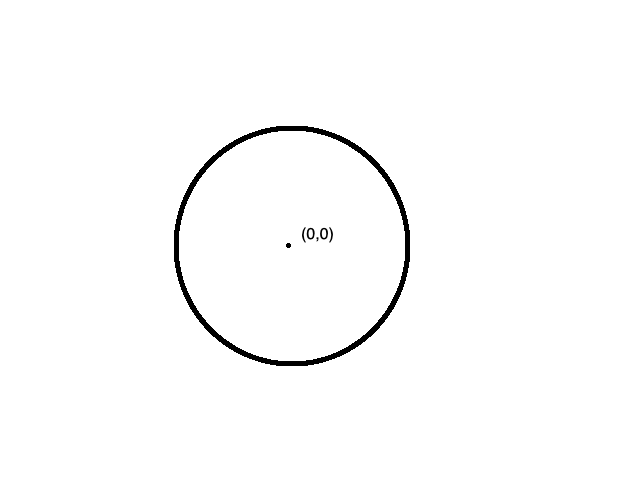
\includegraphics[width=\linewidth]{lec2ex1.png}
	\caption{example 1}        
	\label{fig:ex1}
\end{marginfigure}
The interior, denoted as $A^\circ$ is actually empty, the set is too "thin" to contain an interior, you cannot take an open ball in $\mathbb{R}^2$ around any of it's points. The closure $\bar{A}$ is actually just $A$ itself, since $A^c$ is open in $\mathbb{R}^2$, indeed we can fit an open ball around any point of $A^c$ inside $A^c$, so $A$ is already closed, thus the closure is equal to itself.
\\
$$f^{-1}(\{1\}) \text{ is closed } $$
Another example would be that $A = \{z \colon |z| \leq 1\} \setminus \{1\}$ 
\begin{marginfigure}%
	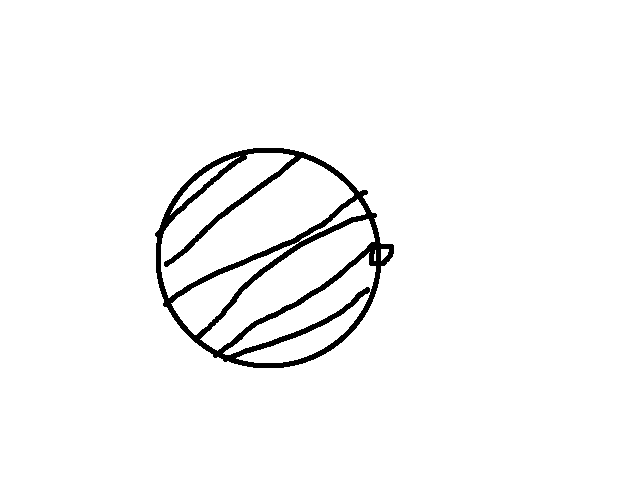
\includegraphics[width=\linewidth]{lec2ex2.png}
	\caption{example 2}        
	\label{fig:ex2}
\end{marginfigure}
The interior of $A$ would just be the open disc $\{z \colon |z| <1\}$, the closure would be the closed disc $\{z \colon |z| \leq 1\}$ 
\begin{lemma}[closedness sequential version]
	Let $A \subseteq X$ which is a t.s. $x \in \bar{A} \iff$ every open neighborhood of $x$ intersects $A$. In other words, $\forall U \in X$ open and $x \in U$ then $U \cap A \neq \emptyset$. A direct consequence of this is that, for any $x \in A$ closed, there exists a sequence $(x_n \colon n \in \mathbb{N})$ in $A$ whose limit is $x$. 
\end{lemma}
An example with the cofinite topology would be $A = [0,1]$, then $\bar{A} = \mathbb{R}$, since $\bar{A}$ smallest closed set that contains $A$, since $\bar{A}$ must contain $A$, then $\bar{A}$ is infinite, the only infinite set that is closed is $\mathbb{R}$. The interior of $A$ is the largest open set 
We prove the lemma 
\begin{proof}
	Assume $x \in \bar{A}$ Let $U$ be an open neighborhood of $x$, then $U^c$ closed. If $U \cap A$ is empty then $A \subseteq U^c$. That means $\bar{A} \cap U^c$ is closed and contains $A$, but $x \notin \bar{A} \cap U^c$, but $x \in \bar{A}$, so $\bar{A} \cap U^c$ is a proper subset of $\bar{A}$ which contradicts the fact that $\bar{A}$ is the smallest set closed in $X$ that contains $A$. 
\end{proof}

\begin{definition}[disconnected]
	$X$ topological space is disconnected if $\exists U,V$ open such that $U \cap V = \emptyset$ and $U\cup V = X$ and $U,V = \emptyset$. 	
\end{definition}
\begin{lemma}
	$X$ is connected if and only if $X$ is not disconnected
\end{lemma}
\begin{lemma}
	$X$ is disconnected if and only if it constains an open subset $U$ which is also closed and $U \neq \emptyset$ or $X$ itself. In other words, $X$ is disconnected if it contains a non trivial clopen subset. 
\end{lemma}
\begin{proof}
	Let $U$ be a non trivial clopen subset, then taking $U^c$ which is open since $U$ is closed, then $U \cup U^c = X$ and $U \cap U^c = \emptyset$, so $U$ and $U^c$ are open sets that partition the space. 
\end{proof}
Example with cofinite topology, it's not disconnected since there can not be any non trivial clopen subset, since a set cannot be finite and have a finite complement as well. 
\begin{lemma}[Some lemmas]
\begin{itemize}
	\item Every interval in $\mathbb{R}$ is connected
	\item $X$ is a topological space (not necessarily connected), $A \subseteq X$, suppose $A$ is connected with the subspace topology, then $\bar{A}$ is connected.
	\item If $f \colon X \to Y$ is continuous and $X$ is connected then $f(X)$ is connected. 
\end{itemize}	
\end{lemma}
\begin{theorem}
	The 8 and the circle is not homeomorphic. 
\end{theorem}
\begin{proof}
	First of all, we need a picture
	\begin{marginfigure}%
		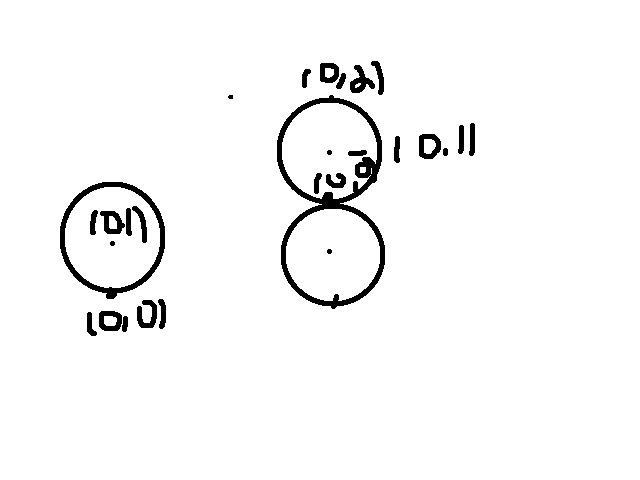
\includegraphics[width=\linewidth]{lec2ex3.png}
		\caption{example 3}        
		\label{fig:ex3}
	\end{marginfigure}
	$x \in X$ be the central point of the $8$, which is $(0,0)$, we have these following claims that are essential in proving the theorem.
	\begin{itemize}
		\item $X \setminus x$ is not connected 
		\item for any $y \in Y$, $Y$ is connected

	\end{itemize}
	Suppose $f : X \to Y$, where $X$ is the figure 8, and $Y$ is the circle, is a homeomorphism, then the function inverse, $f^-1\colon Y \to X$ must be continuous as well. However, 
	$$f^{-1}(Y \setminus \{f(x)\}) = f^{-1}(Y) \setminus f^{-1}(f(x))  = f^{-1}(Y)\setminus \{x\} = X \setminus \{x\}$$
	So the inverse of a connected set is not connected, which leads to a contradiction, since continuous functions must map connected sets to connected sets, thus $f$ is not a homeomorphism
\end{proof}
Proof of claims
\begin{proof}
	$X \setminus \{x\}$ where $x$ is the center point, is disconnected, $U$ is the intersection of $X$ with upper open halfline, $V$ intersection of $X$ with lower open halfline. 
	\begin{marginfigure}%
		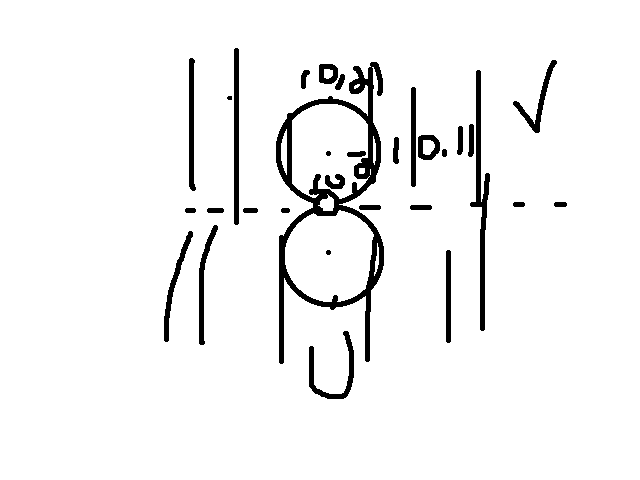
\includegraphics[width=\linewidth]{lec2ex4.png}
		\caption{example 4}        
		\label{fig:ex4}
	\end{marginfigure}
	As in the picture, $U \cap V = \emptyset$, and $U \cup V = X\setminus\{x\}$ 
\end{proof}
Proof $Y\setminus\{y\}$ is connected, since it's homeomorphic to $\mathbb{R}$, we can construct a stereographic projection from the circle to $\mathbb{R}$, draw a line from $(0,2$ to the $x$-axis passing along the point in question.
\end{document}
\begin{definition}[Seperation axioms]
	\begin{enumerate}
		\item $X$ is a topological space, it is called $T_1$ if for all $x,y \in X$, there exists open sets $U,V \in X$ such that $x \in U$, and $y \notin U$, and $y \in V$, and $x \notin V$. 
		\item $X$ is called a "Hausdorff" $T_2$ space if $U \cap V = \emptyset$, along with the conditions for a $T_1$ space. 
	\end{enumerate}	

\end{definition}
Example with $\mathbb{R}$ cofinite topology, we can take any two points say $\{x\}$ and $\{y\}$, it's $T_1$ since we can just take $U = \{x\}^c$ and $V = \{y\}^c$, then $x \in V$, but $y \notin V$, same thing with $U$. But it is not $T_2$, suppose there are two disjoint open sets $U,V$ that contain $x$ and $y$ respectively, then $U^c$ and $V^c$ have to be finite, thus $U$ and $V$ are infinite and unbounded, thus $U \cap V \neq \emptyset$. 
